\subsection{Transfer Functions - Non-Linear System}
\label{sec:TF_non-lin}
On basis on the system response seen in the previous paragraph, it is possible to determine a transfer function for each case of the normalized step. This transfer function is an input-output model of the four tank system. Notice, that the system seen from $u_1$ to $y_1$ and from $u_2$ to $y_2$ can be described by a 1\textsuperscript{st} order system (the general form can be seen in \cref{eq:1st_order_gen}) and the system seen from $u_1$ to $y_2$ and from $u_2$ to $y_1$ is a 2\textsuperscript{nd} order system (the general form can be seen in \cref{eq:2nd_order_gen}). This makes intuitive sense, since the water from u1, needs to go through tank 4, before entering tank 2, and opposite for u2 to tank 1.
\begin{equation}
    \frac{Y(s)}{U(s)}=\frac{K\,e^{-\theta\,s}}{\tau\,s+1}
    \label{eq:1st_order_gen}
\end{equation}
\begin{equation}
    \frac{Y(s)}{U(s)}=\frac{K\,e^{-\theta\,s}}{(\tau_1\,s+1)(\tau_2\,s+1)}
    \label{eq:2nd_order_gen}
\end{equation}
$K$ is the gain of the system which is the steady state value seen in each normalized step. $\theta$ is the time delay, which in the given case is 0. $\tau$ is the time constant of the system. \\
The transfer functions describes a linear system, and therefore the model is only valid close to the linearisation. In the following analysis, the step response of 10\% is evaluated. The system is evaluated when no noise is present and the disturbance is constant at $250\,[cm^3/s]$. The estimated transfer functions is determined to be:
\begin{equation}
    \begin{bmatrix}
        Y_1(s)\\
        Y_2(s)
    \end{bmatrix}
    =
    \begin{bmatrix}
        \frac{0.2083}{138\,s+1} & \frac{0.1144}{(90\,s+1)(138\,s+1)}\\ 
        \frac{0.1686}{(80\,s+1)(173\,s+1)} & \frac{0.2736}{153\,s+1} 
    \end{bmatrix}
    \begin{bmatrix}
        U_1(s)\\
        U_2(s)
    \end{bmatrix}
\end{equation}
\begin{figure}[H]
    \centering
    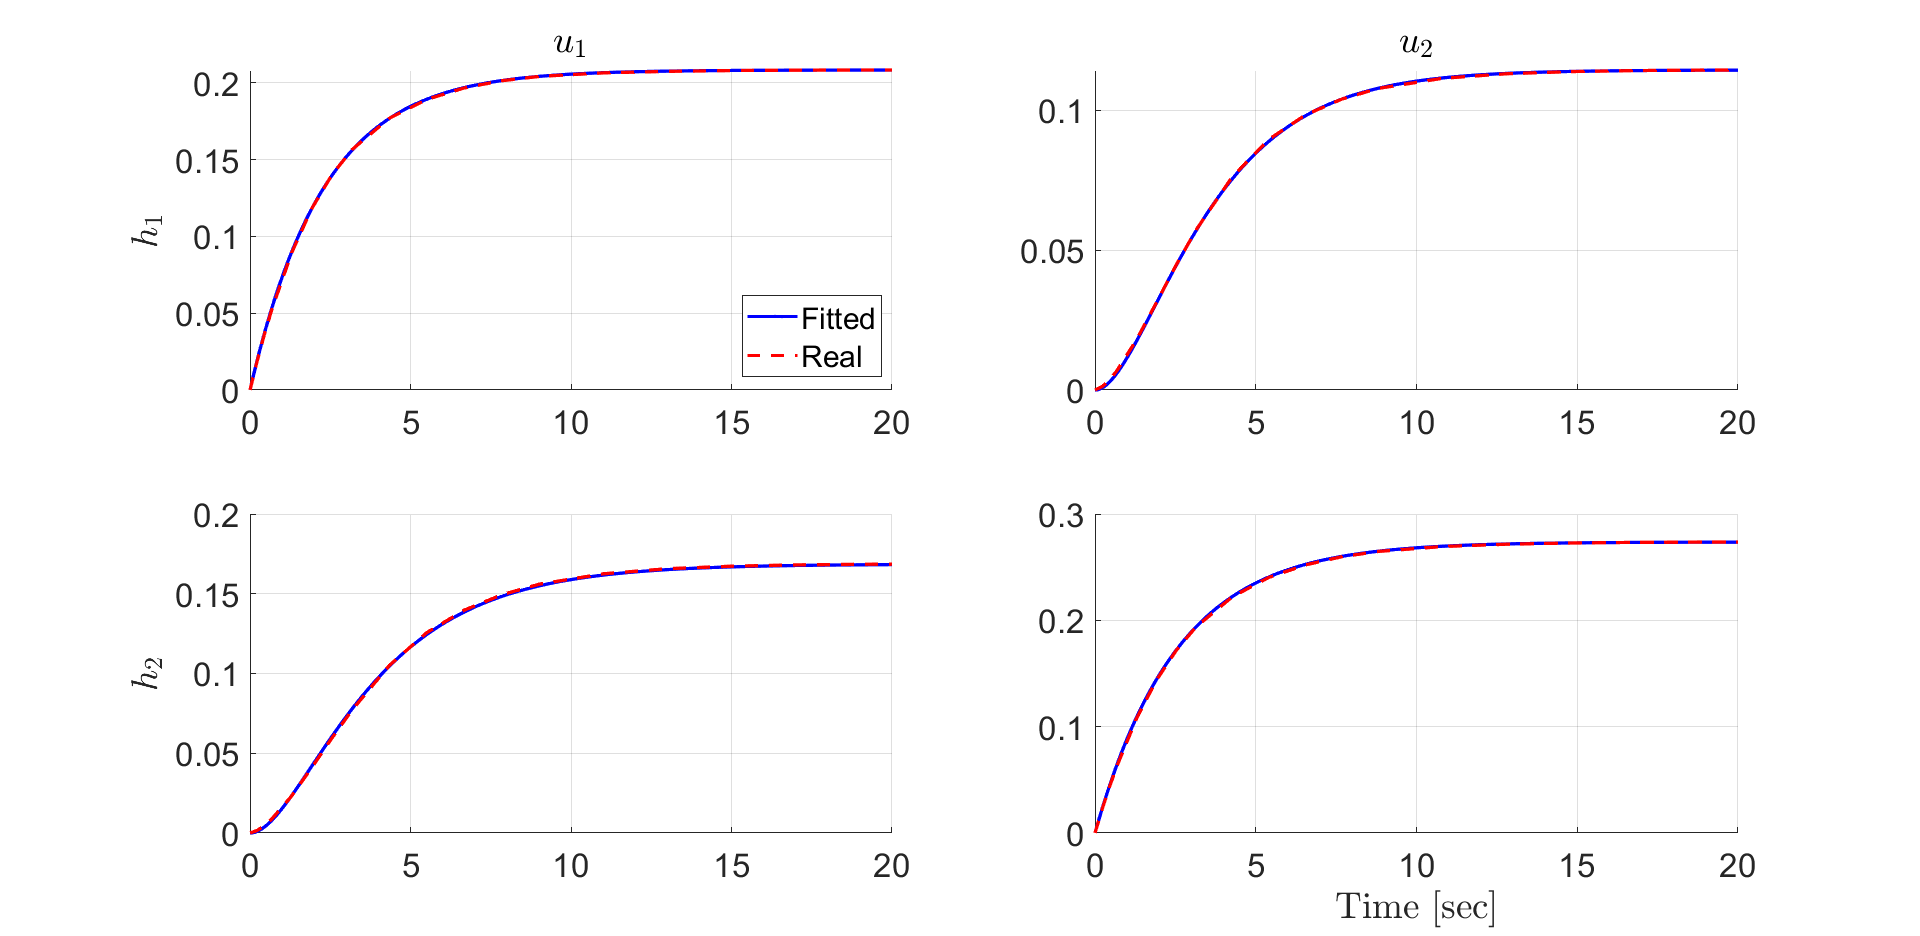
\includegraphics[width=1\textwidth]{Figures/Pr3.4_TF_fit.png}
    \caption{Comparison of transfer function and real response}
    %\label{fig:norm}
\end{figure}